\subsection{W\"urstchen}
In Section~\ref{heading:subsection:stable_diffusion}, we describe the approach
of a \emph{Latent Diffusion Model} (LDM) which was introduced,
by Rombach et al.~\cite{rombach2022stablediffusion} in 2022. The LDM methods
generate images by denoising a noisy latent image gradually step by step. To
conduct the reduction of noise and the introduction of semantics, the LDM takes
in an encoding of a text-prompt, called token or embedding, and utilizes it for
each diffusion step. Lastly, the latent representation is decoded into the
pixel space. By mostly navigating in low dimensional latent spaces and
using the U-Net to gradually introdue semantics into the representation, this
approach is able to yield high resolution images~\cite{rombach2022stablediffusion}.
This improvement in image quality has a disadvantage: the time the models take
to train. For example, an important model is Stable Diffusion (SD), the version
1.4 takes 150,000 GPU hours~\cite{rombach2022sd_1_4} while version 2.1 which
grants an upgrade in image quality has a further increased training time of
200,000 GPU hours~\cite{rombach2023sd_2_1}. A high image resolution comes with
an increased image complexity leading to more data-intensive training and
high computational costs. Thus, Pernias et al.~\cite{pernias2024wrstchen}
introduce \emph{W\"urstchen}. An approach that aims to decrease the training
time and computational cost, by splitting the training process into three parts
and mostly computing in small latent spaces.

This section aims to describe the methods used by W\"urstchen based on the work
of Pernias et al.~\cite{pernias2024wrstchen}. First, we describe the VQGAN by
Esser et al.~\cite{esser2021tamingtransformershighresolutionimage} as this is
the model that is the foundation for Stage A of W\"urstchen. Then, we continue
to shed light onto the general structure and the image generation process. Finally, we
describe the training processes of each W\"urstchen stage as Pernias et al.
provide them.
\subsubsection{VQGAN}
\label{sec:wuerstchen:VQGAN}
The \emph{Vector Quantized Generative Adversarial Network} (VQGAN) was
introduced by Esser et al.~\cite{esser2021tamingtransformershighresolutionimage}
in 2021 and builds on the \emph{Vector Quantized Variational Autoencoder}
model~\cite{vdOord2017NeuralDiscreteRepresentationLearning}. The VQGAN combines
the strengths of \emph{Convolutional Neural Networks} (CNNs) in exploiting local 
features and the strength of autoregressive transformer architectures
to model long-range relations in generated images. Esser et al. introduce
several CNNs to the VQGAN for the training procedure. First, the Encoder CNN
compresses an image $x$ into the compressed version $\hat{z}$. Next,
the VQGAN utilizes the quantization $\boldsymbol{q}[\cdot]$ using a
perceptually rich and discrete codebook $\mathcal{Z}$ to create the quantized
latent representation,
\begin{equation}
    z_{\boldsymbol{q}} = \boldsymbol{q}(\hat{z}) :=\underset{z_{\boldsymbol{k}}\in\mathcal{Z}}{\arg\min}||\hat{z}_{ij} - z_{\boldsymbol{k}}||,
\end{equation}
by replacing the spatial representation $\hat{z}_{ij}$ with the closest
codebook entry $z_{\boldsymbol{k}}$. The latent representation
$z_{\boldsymbol{q}}$ is a sequence of the entries of the codebook $\mathcal{Z}$.
Then, the Decoder CNN reconstructs the image $x$ using the quantized latent
representation $z_{\boldsymbol{q}}$. Finally, to create a rich codebook
a patch-based discriminator CNN is introduced to find the differences between
the real and reconstructed images. An autoregressive transformer model then
makes use of the codebook to generate high-resolution synthetic images.
\subsubsection{W\"urstchen Structure and Image Generation}
\begin{figure}[t]
    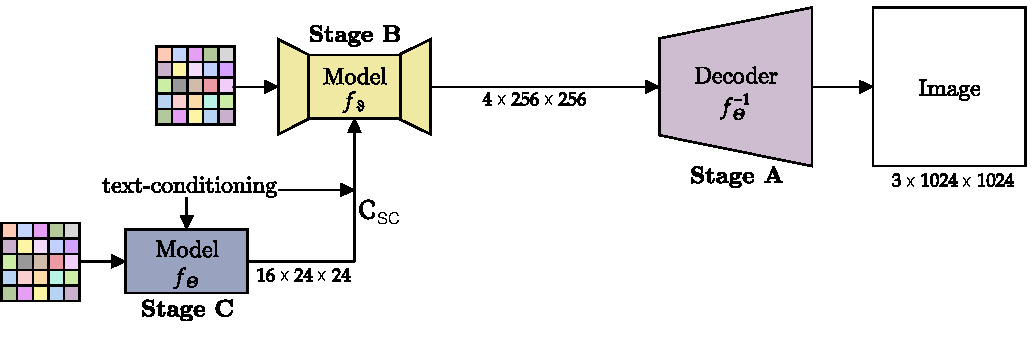
\includegraphics[width=\textwidth]{assets/wuerstchen_arch.pdf}
    \caption{Visualization of the W\"urstchen architecture, introduced by
        Pernias et al.~\cite{pernias2024wrstchen}. It shows that the first stage C
        creates a highly compressed representation from noise and text-conditioning.
        Both this representation and the text-prompt are then utilized as conditionings by stage B
        to create a higher dimensional latent representation. Lastly, the decoder
        in stage A generates an image from this latent representation.}
    \label{fig:wuerstchen:arch}
\end{figure}
In 2024, Pernias et al.~\cite{pernias2024wrstchen} introduce \emph{W\"urstchen}.
With this method, they aim to decrease the computational cost and training
time of image generation models which are based on latent diffusion~\cite{rombach2022stablediffusion}.
Figure~\ref{fig:wuerstchen:arch} illustrates the structure of W\"urstchen which
includes three stages. The first stage, Stage C, comprises a
text-conditional diffusion model $f_\Theta$ that operates on a low-dimensional
latent space with a compression ratio of 42:1. In this stage, the image generation 
pipeline begins by taking latent random noise
$\boldsymbol{X}_{\text{SC}, \tau_C} = \mathcal{N}(0, \boldsymbol{\text{I}})$ and
using the DDPM algorithm by Ho et al.~\cite{ho2020denoisingdiffusionprobabilisticmodels} to iteratively
sample the Semantic Compressor (see Section~\ref{sec:wuerstchen:training})
latent representations on text-conditioning to generate the latent representation
$\bar{\boldsymbol{X}}_{\text{SC}}\in\mathbb{R}^{16\times24\times24}$. Due to
the low dimensionality of the latent space, $f_\Theta$ does not utilize the
typical U-Net structure as the authors decided that any downsampling would do
harm to the image quality. The next stage, Stage B, employs a diffusion model
$f_\vartheta$, utilizing the U-Net architecture. It is conditioned on both the
text-prompt and the embeddings $\mathcal{C}_{\text{SC}}$ of the flattened
$\bar{\boldsymbol{X}}_{\text{SC}}$ from Stage C. This model generates a
higher-dimensional latent representation
$\tilde{\boldsymbol{X}}\in\mathbb{R}^{4\times256\times256}$ by again employing
the DDPM algorithm. The latent space in which $\tilde{\boldsymbol{X}}$ lives
has a compression ratio of 4:1 and is created during the training process by a
VQGAN. Stage A of W\"urstchen consists of the decoder $f_\Theta^{-1}$ which is
part of the same VQGAN. The decoder translates the latent representation
$\tilde{\boldsymbol{X}}$ to the final image,
\begin{equation}
    \bar{\boldsymbol{X}} = f_\Theta^{-1}(\tilde{\boldsymbol{X}}),
\end{equation}
which lives in the pixel space with $\bar{\boldsymbol{X}}\in\mathbb{R}^{3\times1024\times1024}$.
Pernias et al. train each of these stages separately, which we describe in the
following section.
\subsubsection{Training}
\label{sec:wuerstchen:training}
The preceding section, provides an overview of the architecture and structure
of W\"urstchen.
In order to train the model in a more efficient manner, Pernias et
al.~\cite{pernias2024wrstchen} introduce a split training. This approach enables
them to mainly train in low-dimensional latent spaces, which thus yields
performance enhancements. Pernias et al. perform the training in a reverse order
compared to the image generation process (see Figure~\ref{fig:wuerstchen:arch}).
The reason for this are the dependencies between Stage A and Stage B, and Stage B and Stage C.
First, they train Stage A which defines the latent space (4:1) through its VQGAN.
Following, Stage B learns to reconstruct this latent space using embeddings in a
lower dimensional latent space (42:1) which are produced by a semantic compressor.
Finally, Stage C trains to reconstruct the latent space of the semantic
compressor using text-conditioning. The following paragraphs shed light on the methods
of Pernias et al. at a greater detail.
\begin{figure}[t]
    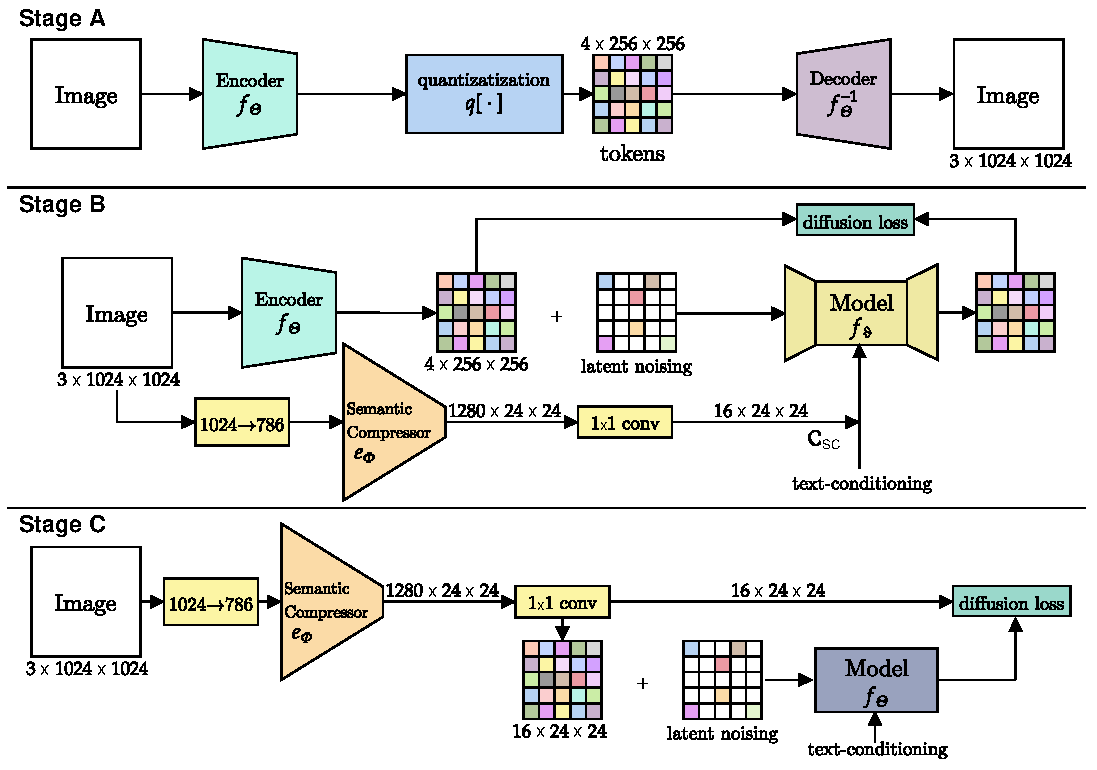
\includegraphics[width=\textwidth]{assets/wuerstchen_training.pdf}
    \caption{Visualization of the training processes of each W\"urstchen stage~\cite{pernias2024wrstchen}.
        On top the training of Stage A followed by Stage B and finally by stage C.
        The training processes of Stages B and C utilize diffusion losses while
        Stage A is trained as a VQGAN.}
    \label{fig:wuerstchen:training}
\end{figure}

\paragraph*{Stage A} The last stage in the image generation pipeline consists of a decoder
$f_{\Theta}^{-1}$ and translates the latent representation produced by Stage B into
the pixel space. This decoder is part of a VQGAN and Pernias et al. train it as
Esset et al.~\cite{esser2021tamingtransformershighresolutionimage} describe.
We touch on this process in Section~\ref{sec:wuerstchen:VQGAN}. During training,
first an encoder $f_{\Theta}$ compresses an image $\boldsymbol{X}\in\mathbb{R}^{3\times1024\times1024}$. Then the compressed image is
quantized using a codebook yielding a latent representation $\boldsymbol{X}_q\in\mathbb{R}^{4\times256\times256}$ of the image with,
$\boldsymbol{X}_q = f_{\Theta}(\boldsymbol{X}).$
Finally, the decoder $f_{\Theta}^{-1}$ reconstructs the image from the latent.
The decoder and encoder are supposed to fulfill the equation,
\begin{equation}
    f_{\Theta}^{-1}(f_{\Theta}(\boldsymbol{X})) = f_{\Theta}^{-1}(\boldsymbol{X}_q) \approx \boldsymbol{X}.
\end{equation}
During training the encoder, the decoder and the codebook are defined. The
encoder defines the latent space with a 4:1 compression ratio, which is
the codomain of the next stage.

\paragraph*{Stage B} This stage reconstructs the latent space defined by the
VQGAN in the training process of Stage A. Therefore, the encoder $f_{\Theta}$
is used to compress the image but without the quantization from the preceding stage.
After noising, the representation $\tilde{\boldsymbol{X}}_t\in\mathbb{R}^{4\times1256\times256}$
is given to the model $f_\vartheta$. For
conditioning Stage B uses both the text embeddings and the results of a
\emph{semantic compressor} $e_{\Phi}$. This semantic compressor mimics Stage C and will be
the foundation of Stage C's training process.

The semantic compressor is a feature extractor of any kind that is supposed to
compress an image to a high degree. The authors advise to choose a model with a
good feature representation and small network size in order to fasten the training
precess of both Stages B and C. Additionally, they mention the size of the
feature space, as too few dimensions would lead to a loss of detail, while to
many dimensions can have a great impact on the computation costs and time. For
these reasons, Pernias et al. chose the CNN, ImageNet1k pre-trained EfficientV2 (S)~\cite{Tan2021EfficientNetV2}.
The semantic compressor gets a bicubic interpolated version of the image and
produces its highly compressed version. Afterward, a $1\times1$ convolution is
applied to reduce the depth and further compress the latent representation $\mathcal{C}_{\text{SC}}\in\mathbb{R}^{16\times24\times24}$.

The embeddings $\mathcal{C}_{\text{SC}}$ of the semantic compressor and the
text-conditioning $\mathcal{C}_{\text{text}}$ are both implemented into the training process using Cross-Attention~\cite{vaswani2023attentionneed}.
Pernias et al. add noise to $\mathcal{C}_{\text{SC}}$ and randomly drop it to
sample with classifier-free-guidance~\cite{ho2022classifierfreediffusionguidance}.
Using both the noised latent representation of the encoder $f_\Theta$ and the
conditioning, the model $f_\vartheta$ trains with the standard diffusion
procedure as we discuss in Section~\ref{sec:stabel_diffusion:training}.

\paragraph*{Stage C} The last stage is supposed to reconstruct the latent space
defined by the semantic compressor $e_\Phi$. Thus, the embeddings
$\mathcal{C}_{\text{SC}}$ are generated as explained for Stage B. Pernias et
al. add a weighted noise to the latent representation
$\boldsymbol{X}_{\text{SC}} = \mathcal{C}_{\text{SC}}$ generated by $e_\Phi$,
\begin{equation}
    \boldsymbol{X}_{\text{SC}, t} = \sqrt{\bar{\alpha}_t}\cdot\boldsymbol{X}_{\text{SC}}+\sqrt{1-\bar{\alpha}_t}\cdot\epsilon,
\end{equation}
with $\bar{\alpha}_t$ defined by a cosine schedule~\cite{Nichol2021ImprovedDenoisingDiffusionProbabilisticModels}.
The model takes $\boldsymbol{X}_{\text{SC}, t}$, $\mathcal{C}_{\text{text}}$ and
the time step $t$ as an input and predicts the error,
\begin{equation}
    \bar{\epsilon} = \frac{\boldsymbol{X}_{\text{SC}, t} - \boldsymbol{A}}{|1-\boldsymbol{B}| + 1e^{-5}} \quad \text{with} \quad \boldsymbol{A}, \boldsymbol{B} = f_\Theta(\boldsymbol{X}_{\text{SC}, t},\mathcal{C}_{\text{text}}, t).
\end{equation}
As the authors mention, they found this change of objective to yield a more
stable training process. The text-embeddings are produced using
CLIP-H~\cite{Ilharco2021OpenCLIP} and are dropped 5\% of the times. In the same
way as the Stage B model, the model $f_\Theta$ is trained using the diffusion
procedure, while conditioning is applied after each block using cross-attention.